\documentclass{article}

\usepackage{amsmath}
\usepackage{amssymb}
\usepackage{chemfig}
\usepackage{mathtools}
\usepackage{listings}
\usepackage{wrapfig}
\usepackage{color}
\usepackage{float}
\usepackage{caption}
\usepackage{subcaption}
\usepackage{multicol}
\usepackage{paralist}
\usepackage{tcolorbox}
\usepackage{braket}
\usepackage[framemethod=TikZ]{mdframed}
\usepackage[english]{babel}
\usepackage[utf8x]{inputenc}
\usepackage[colorinlistoftodos]{todonotes}
\usepackage{esint}
\usepackage{hyperref}

\title{Algorithmic Theory}
\date{2019-01-01}
\author{Animesh Sinha; Gaurang Tandon; Arpan Dasgupta; }

\lstdefinestyle{shared}{
    belowcaptionskip=1\baselineskip,
    breaklines=true,
    xleftmargin=\parindent,
    showstringspaces=false,
    basicstyle=\fontsize{10}{6}\ttfamily,
}
\lstdefinestyle{cpp}{
	style=shared,
    language=C++,
    keywordstyle=\bfseries\color{green!40!black},
    commentstyle=\itshape\color{red!80!black},
    identifierstyle=\color{blue},
    stringstyle=\color{purple!40!black},
}
\lstdefinestyle{java}{
    style=shared,
    language=Java,
    keywordstyle=\bfseries\color{green!40!black},
    commentstyle=\itshape\color{purple!40!black},
    identifierstyle=\color{blue},
    stringstyle=\color{orange},
}
\lstdefinestyle{py}{
    style=shared,
    language=Python,
    keywordstyle=\bfseries\color{green!40!black},
    commentstyle=\itshape\color{purple!40!black},
    identifierstyle=\color{blue},
    stringstyle=\color{orange},
}
\lstdefinestyle{txt}{
    style=shared,
}
\lstset{escapechar=@}

\newcounter{theo}[section]\setcounter{theo}{0}
\renewcommand{\thetheo}{\arabic{section}.\arabic{theo}}
\newenvironment{theorem}[2][]{%
\refstepcounter{theo}%
\ifstrempty{#1}%
{\mdfsetup{%
frametitle={%
\tikz[baseline=(current bounding box.east),outer sep=0pt]
\node[anchor=east,rectangle,fill=blue!20]
{\strut Theorem~\thetheo};}}
}%
{\mdfsetup{%
frametitle={%
\tikz[baseline=(current bounding box.east),outer sep=0pt]
\node[anchor=east,rectangle,fill=blue!20]
{\strut Theorem~\thetheo:~#1};}}%
}%
\mdfsetup{innertopmargin=10pt,linecolor=blue!20,%
linewidth=2pt,topline=true,%
frametitleaboveskip=\dimexpr-\ht\strutbox\relax
}
\begin{mdframed}[]\relax%
\label{#2}}{\end{mdframed}}


\newcounter{prf}[section]\setcounter{prf}{0}
\renewcommand{\theprf}{\arabic{section}.\arabic{prf}}
\newenvironment{proof}[2][]{%
\refstepcounter{prf}%
\ifstrempty{#1}%
{\mdfsetup{%
frametitle={%
\tikz[baseline=(current bounding box.east),outer sep=0pt]
\node[anchor=east,rectangle,fill=red!20]
{\strut Proof~\theprf};}}
}%
{\mdfsetup{%
frametitle={%
\tikz[baseline=(current bounding box.east),outer sep=0pt]
\node[anchor=east,rectangle,fill=red!20]
{\strut Proof~\thetheo:~#1};}}%
}%
\mdfsetup{innertopmargin=10pt,linecolor=red!20,%
linewidth=2pt,topline=true,%
frametitleaboveskip=\dimexpr-\ht\strutbox\relax
}
\begin{mdframed}[]\relax%
\label{#2}}{\end{mdframed}}


\newcounter{exm}[section]\setcounter{exm}{0}
\renewcommand{\theexm}{\arabic{section}.\arabic{exm}}
\newenvironment{example}[2][]{%
\refstepcounter{exm}%
\ifstrempty{#1}%
{\mdfsetup{%
frametitle={%
\tikz[baseline=(current bounding box.east),outer sep=0pt]
\node[anchor=east,rectangle,fill=green!20]
{\strut Example~\theexm};}}
}%
{\mdfsetup{%
frametitle={%
\tikz[baseline=(current bounding box.east),outer sep=0pt]
\node[anchor=east,rectangle,fill=green!20]
{\strut Example~\thetheo:~#1};}}%
}%
\mdfsetup{innertopmargin=10pt,linecolor=green!20,%
linewidth=2pt,topline=true,%
frametitleaboveskip=\dimexpr-\ht\strutbox\relax
}
\begin{mdframed}[]\relax%
\label{#2}}{\end{mdframed}}


\newcounter{def}[section]\setcounter{def}{0}
\renewcommand{\thedef}{\arabic{section}.\arabic{def}}
\newenvironment{definition}[2][]{%
\refstepcounter{def}%
\ifstrempty{#1}%
{\mdfsetup{%
frametitle={%
\tikz[baseline=(current bounding box.east),outer sep=0pt]
\node[anchor=east,rectangle,fill=yellow!20]
{\strut Statement~\thedef};}}
}%
{\mdfsetup{%
frametitle={%
\tikz[baseline=(current bounding box.east),outer sep=0pt]
\node[anchor=east,rectangle,fill=yellow!20]
{\strut Statement~\thetheo:~#1};}}%
}%
\mdfsetup{innertopmargin=10pt,linecolor=yellow!20,%
linewidth=2pt,topline=true,%
frametitleaboveskip=\dimexpr-\ht\strutbox\relax
}
\begin{mdframed}[]\relax%
\label{#2}}{\end{mdframed}}


\title{Optimizing Sewage Structures in a City, and be Resillient in Floods}
\author{Animesh Sinha, Bhuvanesh Sridharan, Kalp Shah, Arpan Dasgupta}

\begin{document}
\pagenumbering{arabic}

\maketitle

\begin{figure}[H]
    \centering
    \begin{subfigure}[b]{0.2\textwidth}
        
\includegraphics[width=\linewidth]{img-iiit-logo.jpeg}
    \end{subfigure}
    \begin{subfigure}[b]{0.25\textwidth}
        
\includegraphics[width=\linewidth]{img-pwc-logo.jpg}
    \end{subfigure}
\end{figure}

\section{What the Problem is?}

\emph{"More important than stopping the floods themselves is to prevent us from flooding toxic material into them."}

Drain flooding is a cause of so much pollution and so many diseases. Millions of people swimming in what seems to be safe waters cause rashes and other diseases, the effects on aquatic life are a lot more severe. They are the carriers of infection. Even when there are no large-scale floods, small drainage cloggages are capable of causing great damage to our efforts against pollution.

\emph{Drains are the folly of Floods, Floods are the folly of Drains}
Drains and Floods have never worked well together, they only worsen the situation caused by each other. Here we will endeavour to design a drainage system which, instead of spilling toxins, will keep them separate from the floods and aid the flood waters get rapidly flushed away, returned in part to land and water bodies.

\section{Core Cases}

\subsection{No Flood Situation - Attempt Water Recharge}

When there are no floods, we want to keep our Sewage Treatment Plants runnning at minimum load, and significantly more importantly, we want to be able to allow the \textbf{maximum amount of water to be recharged into the land without allowing the contaminants in the water to flow off}.

\begin{equation*}
    cost = max (x \times y) \;\;st.\;x + y = f 
\end{equation*}
We define a metric "cost" which we want to lower for our model. 

\subsection{Managable Flood - Not let the Streets Flood}

If the flood can be handled by our network of drains, we would simply have it handled. Rainwater would go into the cleaner channels, and would have ample opportunity of flowing back into the earth. The network can even be pumped if it's in a low lying area. In any case, we DO NOT let the flood water get mixed and spill out the Sewage.

But before we can manage a flood, we must predict if the flood is managable or not. This needs an estimation of the future values of rainfall and drain output, which we compute approximately using a Neural Net regressor.

\subsection{Extreme Floods - Keep the Toxic Stuff out}

When we have a major flood we cannot contain, we have to ensure that our toxic waste (drugs and chemicals, heavy metals, pesticides, insecticides, human waste, etc), and we must not let any of this flow out into the floods. Therefore, once our predictor states that we can no longer handle the load, we cut-off the \textbf{Minimum Spanning Tree} of the city graph for toxic waste. All the rest, the maximum weighted set that is not essential for connection of houses to the waste management plant, is used for routing the Rainwater around.



\section{Cost Analysis}

\subsection{The Minimal Cost Solution}

The minimal solution \textbf{only requires us to install the sensors and the ball valves} which are driven by a motor to route the water in different ways. A single sensor-actuator setup is the minimal we need to get any IoT solution off the ground.
This works with any pre-existing drain graph, therefore, the initial costs of this would not overshoot any smart-city budgets.

\subsection{Expanding to an Extensive Solution}

If we build over the whole city, we would like to have a full redundant network in parallel with our system, integrated withing and only separated by a semi permeable boundary. This would still cost well below twice the current cost of builing the drainaige system, which seeing it's utility and potential is reasonable.

\subsection{Civil Engineering Benefits}

We gain control over the flow network, in particular over the places of the network that have dense, viscous sewage. This allows us to have more targetted deployment of Civil Engineering solutions.
\begin{itemize}
    \item Mud and Particulate matter sticking to gutters is \textbf{the big cause of Drain Clogging}. Since the particulate matter will be routed to one place to minimize the cost function, we can use teflon coatings in our pipes, which otherwise would be very cost inefficient.
    \item Pumping water under high pressure to clear out / force water up some high-sewage drain pipes.
\end{itemize}
and there are many other applications which would be much more cost effective this way.

\section{IoT Sensors and Actuators}

\subsection{List of Sensors}

We have to measure the velocity of flow, and the quality of water.
This requires:
\begin{itemize}
    \item Flow velocity sensors (small Fan Based solutions)
    \item Light Transmittivity based Particulate Matter sensors
\end{itemize}
Hall effect sensors may be more compact and better at measuring flow velocity.

\subsubsection{Bernoulli Detection of Cloggage}

Meshes are a standard in the in-put of Drains. But small particulate mud is the usual cause of cloggages in Drains. Finding out the exact location of these in smart drains is key, and can be done using Flow sensors directly at no extra cost.
Since, by the law of continuity, $v_1 A_1 = v_2 A_2$, so if we know that velocity has increased in a single pipe, effective area has decreased. And if water flow falls significantly, we also detect a clog.

\subsection{Actuator}

All we need to do is Reroute water, we use motorized gate valves for that. This constantly moving bent should also defend against clogging.

We might also have some recharge well infrastructure to return water back to the earth, specially on the cleaner channels.

\subsection{Software}

The IoT sensors/actuators will need to be connected to the internet and have their data stored on the cloud. This would allow rapid live training of ML, and better flood prediction and preemptive actutation.


\section{Algorithmic Facts and Proof of Concepts}

\subsection{The Cut Algorithm for Handing Floods}

We know that any cut of the Graph the allows water to flow exclusively from an unflooded are to a flooded are is invalid, and we must block all the paths that run across the cut.

\begin{definition}[Max-Cut Recursive Algorithm]{larget-cut-recursion}
    The set of edges corresponding to the largest cut (in number of nodes) of the graph and allowing positive flow from non-flooded to flooded regions is the set of edges that need to be closed. This breaks down the graph into two, so we can now recurse.
\end{definition}

\subsection{Augmenting paths for Optimizing Homogeneity}

The cost function denotes the Inhomegeneity in the flow network. Ideally, we would like to keep Dirty (Toxic) and relatively Clean water in separate channels. This would allow us to discharge waste that can be used for water recharge, and others that would immediately require sewage treatment plant. Since every pipe cannot be redundant, we cannot achive perfect separation without doubling the entirity of the current network. However, the following is a measure of the best we can do to maximize Homogeneity (either clean or dirty water but not both). 
\begin{definition}[The Cost function]{def-cost-function}
    \begin{equation*}
        cost = max (x \times y) \;\;st.\;x + y = f 
    \end{equation*}
    This is the measure of heterogeneity, how much of clean and dirty water is mixed, our model should minimize this cost. \textbf{The Net Flow values f must follow the general laws of conservation obeyed by flows.}
\end{definition}
We do this by finding Augmenting paths using a very Dinic like approach and keep maximizing this score. Unlike Dinic's algorithm however, this optimizing is an approximate algorithm, we optimize by iterating, and therefore it's non-terminating. We must stop once we are happy enough with the score we achieved. We shall elaborate on this algorithm in one of the following sections.


\subsection{The Neural Net Regressor}

Here is the exact model we use.
\begin{lstlisting}[basicstyle=Large,style=py]
def build_model():
    # Inputs are: User Index, Time of Day, Time of Year, Zonal Average
    inp_data = tf.keras.layers.Input(shape=(4,))
    prc_data = tf.keras.layers.Dense(5, activation='relu')(inp_data)
    prc_data = tf.keras.layers.Dense(5, activation='relu')(prc_data)
    out_data = tf.keras.layers.Dense(1, activation='relu')(prc_data)
    model = tf.keras.models.Model(inputs=inp_data, outputs=out_data)
    model.compile(loss='mean_squared_error', optimizer='adam')
    return model
    
model = build_model()
history = model.fit(x=in_feed, y=out_feed, epochs=200, validation_split=0.2)
\end{lstlisting}

Following are some figures that show the very promising accuracies of our regressor. 

\begin{figure}[H]
    \centering
    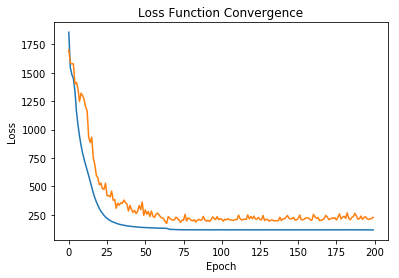
\includegraphics[width=\linewidth]{img-loss-fn-convergence.png}
    \caption{Loss Function Convergence}
    \label{fig:img-loss-fn-convergence}
\end{figure}

Since the Mean Squared Error is as low as about a 100 on both the training and the validation sets (and from the curves it seems that we are still not overfitting, so we can try going further), \textbf{we are accurate in predicting the water consumption of each house down to under \colorbox{yellow}{10 litres} on average}, and this would get us incredibly close on making predictions on the ensamble.

\end{document}
